\section{Auswertung}
\label{sec:Auswertung}

\subsection{Phasenabhängigkeit der Spannung} % (fold)
\label{sub:Phasenabhängigkeit der Spannung}


Am Reference Ausgang des Oszillators ist eine variable Spannung abzugreifen. Am Oszillator Ausgang des Oszillators kann hingegen eine Spannung von $\qty{32}{\volt}$
am Oszilloskop abgelesen werden.
Dieser Wert dient als Referenzwert für $U_{out}$ in den folgenden Messungen.


Einstellungen am Lock-In-Verstärker: Gain am Preamplifier: 20
\begin{figure}
  \centering
  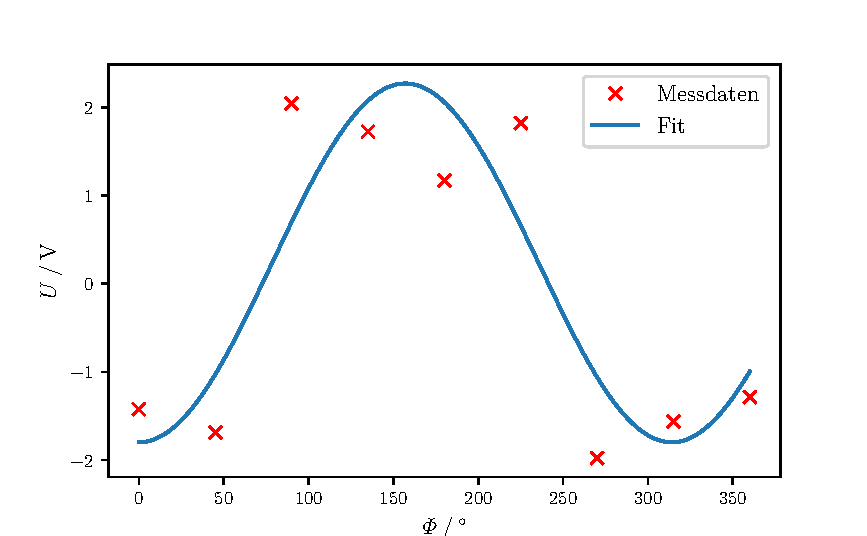
\includegraphics{build/plot1.pdf}
  \caption{Spannungsverlauf am Oszilloskop, in Abhängigkeit von der Phase bei der Messung ohne Noise Generator}
  \label{fig:plot1}
\end{figure}
Uout= 3.2+/-0.8
b= 1.10+/-0.15
c= 0.2+/-0.5


Einstellungen am Lock-In-Verstärker: Gain am Preamplifier: 50
Noise Amplitude $10^-3$
Signal Attentuator $10^-5$

\begin{figure}
  \centering
  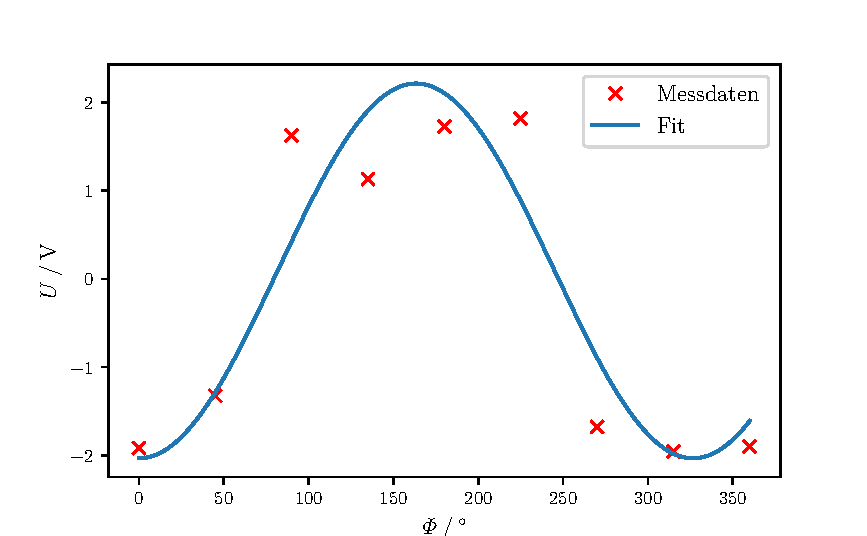
\includegraphics{build/plot2.pdf}
  \caption{Spannungsverlauf am Oszilloskop, in Abhängigkeit von der Phase bei der Messung mit zwischengeschaltetem Noise Generator}
  \label{fig:plot2}
\end{figure}

Uout= 3.4+/-0.6
b= 1.02+/-0.13
c= 0.3+/-0.4

\subsection{Rauschunterdrückung bei einer Photodetektorschaltung} % (fold)
\label{sub:Rauschunterdrückung bei einer Photodetektorschaltung}


\begin{table}[H]
  \centering
  \sisetup{table-format=3.0}
  \begin{tabular}{S S[table-format=3.2]}
    \toprule
    {Abstand der Diode $\mathbin{/} \si{\centi\meter}$} & {$U \mathbin{/} \si{volt}$}\\
    \midrule
    10  &    104.00\\
    15  &    108.90\\
    20  &    107.91\\
    25  &    106.92\\
    30  &    88.11 \\
    35  &    77.22 \\
    40  &    57.42 \\
    45  &    46.53 \\
    50  &    35.64 \\
    55  &    29.70 \\
    60  &    24.75 \\
    65  &    21.78 \\
    70  &    18.81 \\
    75  &    16.83 \\
    80  &    15.84 \\
    85  &    13.86 \\
    90  &    11.88 \\
    95  &    10.89 \\
    100 &    10.89 \\
    105 &    9.90  \\
    110 &    8.91  \\
    115 &    8.91  \\
    120 &    7.92  \\
    125 &    6.93  \\
    130 &    6.93  \\
    135 &    6.93  \\
    140 &    6.93  \\
    145 &    6.93  \\
    150 &    6.93  \\
    \bottomrule
  \end{tabular}
  \caption{Messwerte der Spannung am Photodetektor, sowie Abstand der LED vom Detektor.}
  \label{tab:Diode}
\end{table}
\begin{figure}
  \centering
  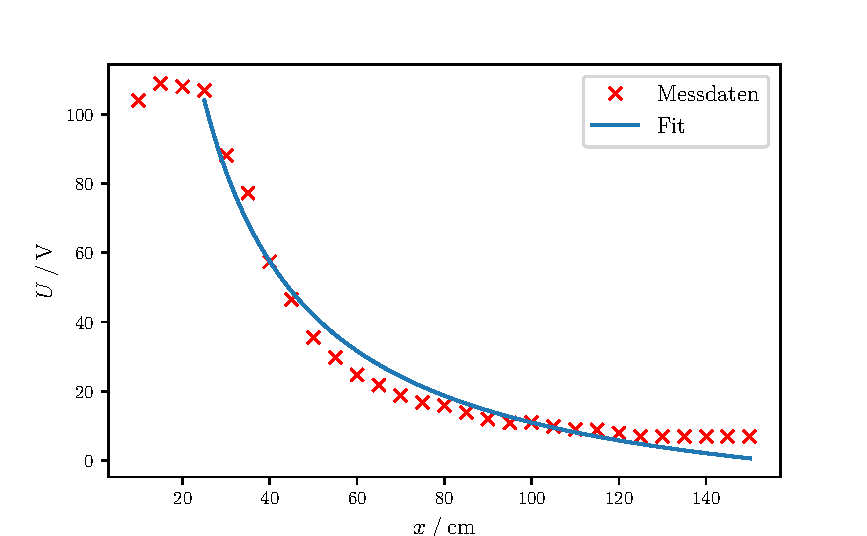
\includegraphics{build/plot3.pdf}
  \caption{Spannungsverlauf am Oszilloskop, in Abhängigkeit vom Abstand der LED zum Photodetektor}
  \label{fig:plot3}
\end{figure}

Regression mit der Funktion $a \cdot \frac{1}{x} +b$ durchgeführt, allerdings erst ab Wert von 25cm, da die Werte davor nicht mit dem Faktor $\frac{1}{x}$ abfallen.
a= (3.10+/-0.10)e+03
b= -20.1+/-1.7

